\documentclass[11pt,letterpaper]{article}
\usepackage[margin=0.8in,top=0.85in,bottom=0.8in]{geometry}
\usepackage[T1]{fontenc}
\usepackage[utf8]{inputenc}
\usepackage{newtxtext,newtxmath,microtype,graphicx,booktabs,longtable,array,tabularx,multirow,xcolor,fancyhdr,lastpage,pdflscape,caption,tocloft,hyperref,colortbl}
\hypersetup{colorlinks=true,linkcolor=black,urlcolor=blue,pdftitle=Reserve Management Plan}
\definecolor{linegray}{HTML}{C8CDD2}
\definecolor{sectionblue}{HTML}{3A5F7D}
\definecolor{softgray}{HTML}{F6F7F8}
\setlength{\headheight}{16pt}
\pagestyle{fancy}
\fancyhf{}
\fancyhead[L]{\footnotesize Ridge Park Luxury Condominiums Owners' Association Inc.}
\fancyhead[R]{\footnotesize January 1, 2026}
\fancyfoot[L]{\footnotesize Reserve Study Report}
\fancyfoot[R]{\footnotesize Page \thepage\ of \pageref{LastPage}}
\setlength{\parindent}{0pt}
\setlength{\parskip}{0.45em}
\renewcommand{\arraystretch}{1.18}

\newcommand{\sectionrule}{\par\vspace{0.2em}{\color{linegray}\rule{\linewidth}{0.6pt}}\par\vspace{0.6em}}
\newcommand{\reportsection}[1]{%
  \par\vspace{0.2em}%
  \addcontentsline{toc}{section}{#1}%
  {{\Large\bfseries\color{sectionblue} #1\par}}%
  \sectionrule
}
\newcommand{\subnote}[1]{\vspace{0.3em}\colorbox{softgray}{\parbox{0.97\linewidth}{\small #1}}\vspace{0.4em}}

\begin{document}

\thispagestyle{empty}
\begin{flushleft}
{\small Board of Directors}\\
{\small Ridge Park Luxury Condominiums Owners' Association Inc.}\\
{\small Los Alamos, New Mexico}
\end{flushleft}

\vspace{0.8em}
Please find attached your reserve study report. This version was generated from association CSV source files using a Python-to-LaTeX workflow so that the report can be reproduced, updated, and audited from the underlying data package.

The report is intended to mirror the structure and feel of a conventional reserve study: a cover page, statement of position, component summaries, annual funding projections, expenditure schedules, and supporting disclosures. The purpose is not to imitate the original preparer's authorship, but to provide a transparent and reusable reporting format driven directly by the uploaded reserve data.

The reserve model remains a planning tool rather than a prediction of exact future outcomes. Actual repair timing, pricing, inflation, and investment returns will differ from the assumptions used here. The goal is to keep the association approximately funded at approximately the right time and to make long-range reserve decisions easier to review.

Sincerely,\\[0.7em]
Brendan J. Gifford\\
Ridge Park Treasurer
\newpage

\thispagestyle{empty}
\begin{center}
\vspace*{1.2cm}
{\LARGE\bfseries Ridge Park Luxury Condominiums Owners' Association Inc.}\\[2.0cm]
{\Huge\bfseries Reserve Management Plan}\\[0.45cm]
{\Large\bfseries Type 1}\\[0.45cm]
{\LARGE\bfseries Reserve Study with Data-Driven Analysis}\\[1.7cm]
{\large\bfseries For 30-Year Projection Period Beginning January 1, 2026}\\[1.0cm]
\IfFileExists{cover_img.png}{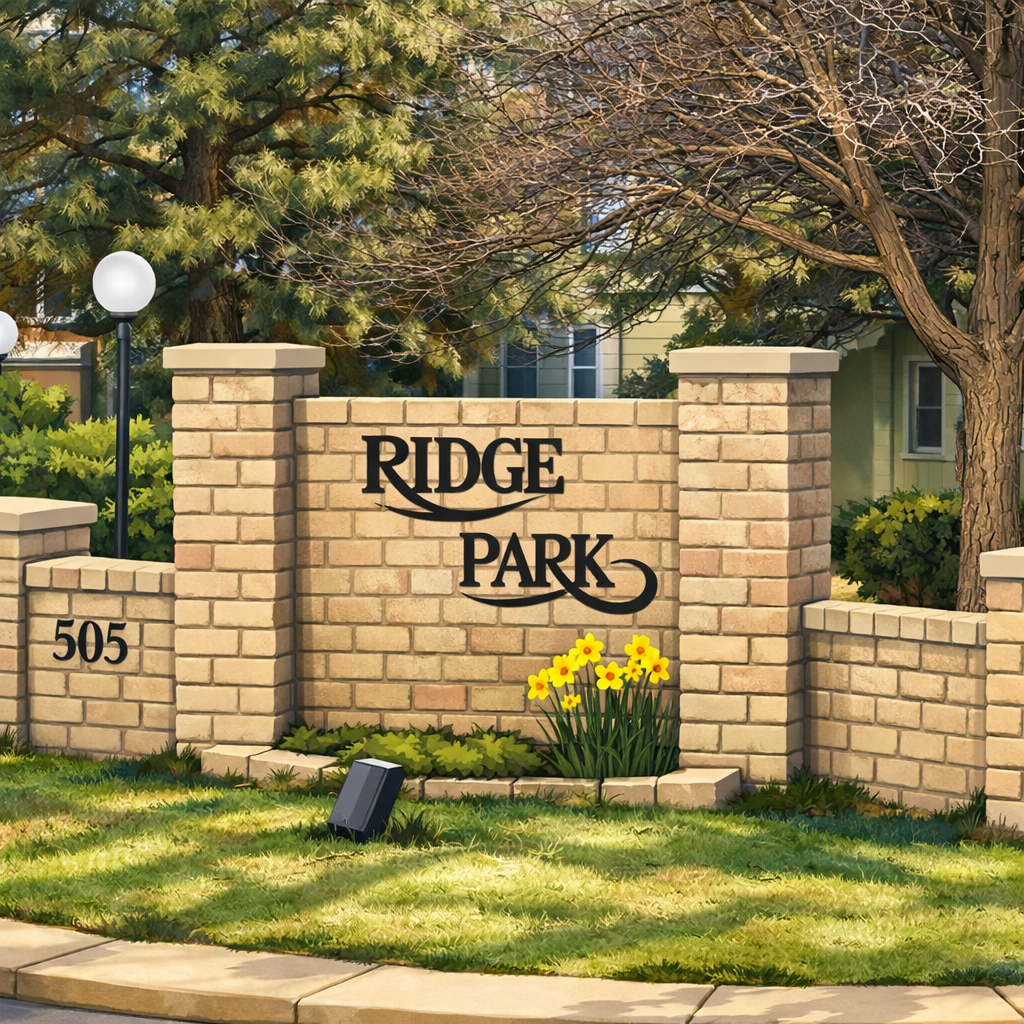
\includegraphics[width=0.68\linewidth]{cover_img.png}}{\vspace{3cm}}
\end{center}
\newpage

\tableofcontents
\newpage

\reportsection{Preparer's Report on Reserve Study}
{\bfseries Description of Engagement and Report}\\
This report was generated from the uploaded CSV data package for the association. The workflow reads the reserve assumptions, component inventory, replacement schedule, annual contribution plan, and reserve cash-flow projection, then renders a formatted LaTeX report designed to resemble a traditional reserve study binder. It is intended as a reproducible reporting layer over the association's source data.

{\bfseries Management's Responsibility}\\
Management remains responsible for the assumptions underlying the reserve model, including inflation, investment return, beginning reserve balance, component scope, useful life estimates, replacement timing, and any planned contribution or special assessment strategy.

{\bfseries Generator Responsibility}\\
The generator's responsibility is limited to organizing the supplied data into financial exhibits, narrative disclosures, and summary schedules. It does not perform a site inspection, engineering opinion, destructive testing, or warranty analysis.

{\bfseries Important Limitations}\\
This report should be read together with the source CSV package. If the underlying source data changes, the PDF should be regenerated so that tables and summary metrics remain aligned with the current model.

\subnote{This document was not prepared by a credentialed professional. It is best treated as a transparent analytical report, not as a substitute for a professional reserve study.}

\newpage
\reportsection{Statement of Position}
\begin{tabularx}{\linewidth}{>{\bfseries}l X}
Projection period: & 2026 to 2055 \\
Type of project: & Reserve Study \\
Number of units: & 138 \\
Location: & Los Alamos, New Mexico \\
Project construction date: & 1984 \\
Analysis date: & January 1, 2026 \\
Report prepared by: & Brendan J. Gifford, Treasurer \\
\end{tabularx}

\vspace{0.8em}
\begin{tabularx}{\linewidth}{X r}
\toprule
Metric & Value \\
\midrule
\rowcolor{blue!12} Current Replacement Cost & \$6,283,484 \\
Future Replacement Cost & \$8,723,989 \\
\rowcolor{blue!12} Current Reserve Fund Balance & \$800,000 \\
Fully Funded Reserve Balance & \$3,426,289 \\
\rowcolor{blue!12} Percent Funded & 23.35 \% \\
Reserve Deficit & \$2,626,289 \\
\rowcolor{blue!12} Reserve Deficit per Unit & \$19,031 \\
Projected Annual Reserve Contribution & \$250,000 \\
\rowcolor{blue!12} Average Annual Reserve Contribution per Unit & \$1,812 \\
Projected Monthly Reserve Contribution & \$20,833 \\
\rowcolor{blue!12} Average Monthly Reserve Contribution per Unit & \$151 \\
\bottomrule
\end{tabularx}

\subnote{First-year reserve contribution: \$250,000. First-year ending balance: \$757,274. Ending balance in the final projection year (2055): \$10,227,048.}

\newpage
\reportsection{Summary of Major Components}
{\small Analysis Date - January 1, 2026 \quad Inflation: 3.00\% \quad Investment: 2.50\% \quad Contribution Factor: 0.00}

\vspace{0.6em}
\begin{tabularx}{\linewidth}{X >{\centering\arraybackslash}p{1.3cm} >{\centering\arraybackslash}p{2.2cm} >{\centering\arraybackslash}p{2.3cm} >{\raggedleft\arraybackslash}p{2.7cm}}
\toprule
Category & Useful Lives & Replacement Years & Remaining Years & Future Cost \\
\midrule
\rowcolor{blue!12} Roofing & 5-30 & 2030-2040 & 4:06-14:06 & \$2,582,679 \\
Exterior Surfaces & 7-30 & 2026-2040 & 0:06-14:06 & \$2,481,562 \\
\rowcolor{blue!12} Asphalt & 3-30 & 2026-2056 & 0:06-30:06 & \$2,071,456 \\
Painting & 3-12 & 2026-2036 & 0:06-10:06 & \$834,324 \\
\rowcolor{blue!12} Balconies-Decks-Stairways & 5-20 & 2026-2031 & 0:06-5:06 & \$431,381 \\
Flooring & 12-20 & 2034 & 8:06 & \$75,081 \\
\rowcolor{blue!12} Renovation & 10-20 & 2029-2039 & 3:06-13:06 & \$63,913 \\
Concrete & 3-25 & 2026-2044 & 0:06-18:06 & \$48,231 \\
\rowcolor{blue!12} Fences-Walls-Gates & 3-25 & 2026-2036 & 0:06-10:06 & \$35,466 \\
Equipment & 7-25 & 2028-2036 & 2:06-10:06 & \$29,002 \\
\rowcolor{blue!12} Doors-Windows & 10 & 2036 & 10:06 & \$24,551 \\
Landscape & 1-8 & 2026-2031 & 0:06-5:06 & \$14,613 \\
\rowcolor{blue!12} Structural & 5-10 & 2026-2028 & 0:06-2:06 & \$12,995 \\
Plumbing & 2-12 & 2026-2031 & 0:06-5:06 & \$7,898 \\
\rowcolor{blue!12} Fire Safety & 5 & 2029 & 3:06 & \$5,545 \\
Signage & 5-20 & 2026-2029 & 0:06-3:06 & \$5,292 \\
\bottomrule
\end{tabularx}

\newpage
\reportsection{Percent Funded - Annual - Ending Balance}
\begin{longtable}{>{\centering\arraybackslash}p{1.4cm} >{\raggedleft\arraybackslash}p{2.6cm} >{\raggedleft\arraybackslash}p{2.7cm} >{\raggedleft\arraybackslash}p{2.0cm}}
\toprule
Year & Ending Balance & Funded Balance & Percent Funded \\
\midrule
\endfirsthead
\toprule
Year & Ending Balance & Funded Balance & Percent Funded \\
\midrule
\endhead
\rowcolor{blue!12} 2026 & \$757,274 & \$3,549,436 & 21.34\% \\
2027 & \$812,144 & \$3,784,463 & 21.46\% \\
\rowcolor{blue!12} 2028 & \$648,132 & \$3,798,324 & 17.06\% \\
2029 & \$635,325 & \$3,957,293 & 16.05\% \\
\rowcolor{blue!12} 2030 & \$341,988 & \$3,828,312 & 8.93\% \\
2031 & \$228,127 & \$3,876,917 & 5.88\% \\
\rowcolor{blue!12} 2032 & \$239,647 & \$4,049,899 & 5.92\% \\
2033 & \$574,956 & \$4,481,720 & 12.83\% \\
\rowcolor{blue!12} 2034 & \$758,217 & \$4,694,369 & 16.15\% \\
2035 & \$753,102 & \$4,646,566 & 16.21\% \\
\rowcolor{blue!12} 2036 & \$207,993 & \$3,982,367 & 5.22\% \\
2037 & \$208,300 & \$3,790,031 & 5.50\% \\
\rowcolor{blue!12} 2038 & \$217,800 & \$3,531,701 & 6.17\% \\
2039 & \$211,567 & \$3,259,362 & 6.49\% \\
\rowcolor{blue!12} 2040 & \$209,106 & \$2,993,022 & 6.99\% \\
2041 & \$815,980 & \$3,341,436 & 24.42\% \\
\rowcolor{blue!12} 2042 & \$1,476,796 & \$3,750,208 & 39.38\% \\
2043 & \$2,305,537 & \$4,334,740 & 53.19\% \\
\rowcolor{blue!12} 2044 & \$3,077,480 & \$4,870,826 & 63.18\% \\
2045 & \$3,948,982 & \$5,486,838 & 71.97\% \\
\rowcolor{blue!12} 2046 & \$3,887,366 & \$5,144,727 & 75.56\% \\
2047 & \$4,428,490 & \$5,388,964 & 82.18\% \\
\rowcolor{blue!12} 2048 & \$4,958,756 & \$5,605,232 & 88.47\% \\
2049 & \$5,600,997 & \$5,916,021 & 94.68\% \\
\rowcolor{blue!12} 2050 & \$6,123,848 & \$6,088,613 & 100.58\% \\
2051 & \$6,585,470 & \$6,188,599 & 106.41\% \\
\rowcolor{blue!12} 2052 & \$7,350,213 & \$6,581,470 & 111.68\% \\
2053 & \$8,216,889 & \$7,057,275 & 116.43\% \\
\rowcolor{blue!12} 2054 & \$9,134,587 & \$7,564,425 & 120.76\% \\
2055 & \$10,227,048 & \$8,226,481 & 124.32\% \\
\bottomrule
\end{longtable}

\newpage
\reportsection{Cash Flow - Annual}
\begin{longtable}{>{\centering\arraybackslash}p{1.1cm} >{\raggedleft\arraybackslash}p{2.0cm} >{\raggedleft\arraybackslash}p{1.9cm} >{\raggedleft\arraybackslash}p{2.1cm} >{\raggedleft\arraybackslash}p{1.9cm} >{\raggedleft\arraybackslash}p{1.7cm} >{\raggedleft\arraybackslash}p{2.0cm}}
\toprule
Year & Begin & Contribution & Special Assess. & Expenditures & Interest & Ending \\
\midrule
\endfirsthead
\toprule
Year & Begin & Contribution & Special Assess. & Expenditures & Interest & Ending \\
\midrule
\endhead
\rowcolor{blue!12} 2026 & \$800,000 & \$250,000 & \$0 & \$313,093 & \$20,367 & \$757,274 \\
2027 & \$757,274 & \$267,616 & \$0 & \$233,110 & \$20,364 & \$812,144 \\
\rowcolor{blue!12} 2028 & \$812,144 & \$285,233 & \$0 & \$468,772 & \$19,527 & \$648,132 \\
2029 & \$648,132 & \$302,849 & \$0 & \$332,699 & \$17,043 & \$635,325 \\
\rowcolor{blue!12} 2030 & \$635,325 & \$320,466 & \$0 & \$627,676 & \$13,874 & \$341,988 \\
2031 & \$341,988 & \$338,082 & \$0 & \$460,390 & \$8,446 & \$228,127 \\
\rowcolor{blue!12} 2032 & \$228,127 & \$355,698 & \$0 & \$351,128 & \$6,950 & \$239,647 \\
2033 & \$239,647 & \$437,870 & \$0 & \$113,410 & \$10,849 & \$574,956 \\
\rowcolor{blue!12} 2034 & \$574,956 & \$520,041 & \$0 & \$354,706 & \$17,926 & \$758,217 \\
2035 & \$758,217 & \$602,212 & \$0 & \$628,148 & \$20,821 & \$753,102 \\
\rowcolor{blue!12} 2036 & \$753,102 & \$684,383 & \$0 & \$1,244,855 & \$15,362 & \$207,993 \\
2037 & \$207,993 & \$766,554 & \$0 & \$773,872 & \$7,625 & \$208,300 \\
\rowcolor{blue!12} 2038 & \$208,300 & \$848,726 & \$0 & \$847,212 & \$7,987 & \$217,800 \\
2039 & \$217,800 & \$853,489 & \$0 & \$867,800 & \$8,077 & \$211,567 \\
\rowcolor{blue!12} 2040 & \$211,567 & \$858,253 & \$0 & \$868,689 & \$7,975 & \$209,106 \\
2041 & \$209,106 & \$863,017 & \$0 & \$270,379 & \$14,236 & \$815,980 \\
\rowcolor{blue!12} 2042 & \$815,980 & \$867,780 & \$0 & \$236,961 & \$29,998 & \$1,476,796 \\
2043 & \$1,476,796 & \$872,544 & \$0 & \$92,092 & \$48,289 & \$2,305,537 \\
\rowcolor{blue!12} 2044 & \$2,305,537 & \$877,308 & \$0 & \$173,822 & \$68,457 & \$3,077,480 \\
2045 & \$3,077,480 & \$903,627 & \$0 & \$121,014 & \$88,889 & \$3,948,982 \\
\rowcolor{blue!12} 2046 & \$3,948,982 & \$930,736 & \$0 & \$1,093,478 & \$101,126 & \$3,887,366 \\
2047 & \$3,887,366 & \$958,658 & \$0 & \$523,446 & \$105,912 & \$4,428,490 \\
\rowcolor{blue!12} 2048 & \$4,428,490 & \$987,417 & \$0 & \$576,584 & \$119,432 & \$4,958,756 \\
2049 & \$4,958,756 & \$1,017,040 & \$0 & \$508,755 & \$133,956 & \$5,600,997 \\
\rowcolor{blue!12} 2050 & \$5,600,997 & \$1,047,551 & \$0 & \$673,589 & \$148,889 & \$6,123,848 \\
2051 & \$6,123,848 & \$1,078,978 & \$0 & \$778,795 & \$161,440 & \$6,585,470 \\
\rowcolor{blue!12} 2052 & \$6,585,470 & \$1,111,347 & \$0 & \$522,837 & \$176,232 & \$7,350,213 \\
2053 & \$7,350,213 & \$1,144,687 & \$0 & \$474,543 & \$196,532 & \$8,216,889 \\
\rowcolor{blue!12} 2054 & \$8,216,889 & \$1,179,028 & \$0 & \$480,188 & \$218,858 & \$9,134,587 \\
2055 & \$9,134,587 & \$1,214,399 & \$0 & \$365,684 & \$243,746 & \$10,227,048 \\
\bottomrule
\end{longtable}

\newpage
\reportsection{Disclosures}
\begin{itemize}
\item This report was generated from current component inventory and condition, projected expenditures, annual contribution schedules, and reserve cash-flow projections.
\item Analysis date: January 1, 2026. Projection horizon: 30 years.
\item Inflation assumption used in the model: 3.00\%.
\item Investment return assumption used in the model: 2.50\%.
\item Beginning reserve balance used in the projection: \$800,000.
\item While component replacement timing and cost estimates are best guesses, actual field conditions may cause different timing or scope.
\item This document is formatted to resemble a conventional reserve study using custom Python-based software designed and written by Brendan J. Gifford rather than from proprietary reserve-study software.
\item Readers should review contribution levels, projected expenditures, and percent-funded results together. No single table should be interpreted in isolation.
\end{itemize}

\newpage
\begin{landscape}
\reportsection{Expenditures Matrix: Years 1--10}
\scriptsize
\setlength{\tabcolsep}{4.0pt}
\begin{tabular}{p{4.2cm}*{10}{r}}
\toprule
Category & 2026 & 2027 & 2028 & 2029 & 2030 & 2031 & 2032 & 2033 & 2034 & 2035 \\
\midrule
\rowcolor{blue!12} Asphalt & \$25,372 &  &  & \$27,725 &  &  &  &  &  & \$397,260 \\
Balconies-Decks-Stairways & \$65,968 & \$60,107 & \$108,208 & \$63,767 & \$65,680 & \$67,651 &  & \$31,205 & \$9,642 & \$19,863 \\
\rowcolor{blue!12} Concrete & \$15,223 &  &  & \$16,635 &  &  & \$18,177 &  &  & \$19,863 \\
Doors-Windows &  &  &  &  &  &  &  &  &  &  \\
\rowcolor{blue!12} Equipment &  &  & \$6,331 &  & \$1,713 & \$3,000 & \$909 &  &  &  \\
Exterior Surfaces & \$68,505 & \$60,107 & \$223,414 & \$74,857 & \$408,360 & \$173,539 & \$181,775 & \$6,241 & \$205,701 &  \\
\rowcolor{blue!12} Fences-Walls-Gates & \$5,074 &  & \$1,615 & \$11,090 &  & \$2,941 & \$3,030 & \$1,872 & \$6,428 & \$3,310 \\
Fire Safety &  &  &  & \$5,545 &  &  &  &  & \$6,428 &  \\
\rowcolor{blue!12} Flooring &  &  &  &  &  &  &  &  & \$75,081 &  \\
Landscape & \$11,671 & \$8,363 & \$8,614 & \$12,753 & \$9,138 & \$12,354 & \$13,936 & \$9,985 & \$10,285 & \$15,228 \\
\rowcolor{blue!12} Painting & \$106,563 & \$104,534 & \$107,670 & \$116,445 & \$114,227 & \$117,653 & \$127,242 &  & \$3,857 & \$6,621 \\
Plumbing & \$5,074 &  & \$5,383 &  & \$5,711 & \$2,824 & \$6,059 &  & \$6,428 &  \\
\rowcolor{blue!12} Renovation &  &  &  & \$2,772 &  & \$8,824 &  &  & \$30,855 &  \\
Roofing &  &  &  &  & \$22,845 & \$60,427 &  & \$64,107 &  & \$166,002 \\
\rowcolor{blue!12} Signage & \$2,030 &  & \$2,153 & \$1,109 &  & \$2,353 &  &  &  &  \\
Structural & \$7,612 &  & \$5,383 &  &  & \$8,824 &  &  &  &  \\
\bottomrule
\end{tabular}
\end{landscape}

\newpage
\begin{landscape}
\reportsection{Expenditures Matrix: Years 11--20}
\scriptsize
\setlength{\tabcolsep}{4.0pt}
\begin{tabular}{p{4.2cm}*{10}{r}}
\toprule
Category & 2036 & 2037 & 2038 & 2039 & 2040 & 2041 & 2042 & 2043 & 2044 & 2045 \\
\midrule
\rowcolor{blue!12} Asphalt &  &  & \$36,175 &  & \$61,404 & \$39,529 &  &  & \$43,195 & \$71,185 \\
Balconies-Decks-Stairways & \$4,092 &  & \$36,175 &  &  &  & \$36,643 & \$41,936 & \$5,183 &  \\
\rowcolor{blue!12} Concrete &  &  & \$21,705 &  &  & \$23,717 &  &  & \$58,924 &  \\
Doors-Windows & \$24,551 &  &  &  &  &  &  &  &  &  \\
\rowcolor{blue!12} Equipment & \$17,049 & \$2,107 &  &  & \$4,421 &  &  & \$5,032 & \$2,592 &  \\
Exterior Surfaces & \$223,957 & \$210,727 & \$217,048 & \$223,560 & \$230,267 &  & \$16,286 & \$25,162 &  &  \\
\rowcolor{blue!12} Fences-Walls-Gates & \$23,869 &  & \$5,788 & \$11,178 &  & \$7,906 &  & \$2,516 & \$12,958 &  \\
Fire Safety &  &  &  & \$7,452 &  &  &  &  & \$8,639 &  \\
\rowcolor{blue!12} Flooring &  &  &  &  &  &  &  &  &  &  \\
Landscape & \$10,911 & \$11,239 & \$16,640 & \$15,649 & \$12,281 & \$18,183 & \$13,029 & \$13,420 & \$19,869 & \$14,237 \\
\rowcolor{blue!12} Painting & \$184,130 & \$140,484 & \$151,934 & \$149,040 & \$153,511 & \$166,022 & \$162,860 &  & \$13,822 &  \\
Plumbing & \$6,820 &  & \$7,235 &  & \$7,676 &  & \$8,143 & \$4,026 & \$8,639 &  \\
\rowcolor{blue!12} Renovation &  &  &  & \$25,188 &  &  &  &  &  &  \\
Roofing & \$736,520 & \$409,315 & \$347,277 & \$434,243 & \$399,129 &  &  &  &  & \$35,592 \\
\rowcolor{blue!12} Signage & \$2,728 &  &  & \$1,490 &  & \$3,162 &  &  &  &  \\
Structural & \$10,229 &  & \$7,235 &  &  & \$11,859 &  &  &  &  \\
\bottomrule
\end{tabular}
\end{landscape}

\newpage
\begin{landscape}
\reportsection{Expenditures Matrix: Years 21--30}
\scriptsize
\setlength{\tabcolsep}{4.0pt}
\begin{tabular}{p{4.2cm}*{10}{r}}
\toprule
Category & 2046 & 2047 & 2048 & 2049 & 2050 & 2051 & 2052 & 2053 & 2054 & 2055 \\
\midrule
\rowcolor{blue!12} Asphalt &  & \$47,200 &  &  & \$51,577 & \$254,994 & \$262,644 & \$326,883 & \$278,639 & \$286,998 \\
Balconies-Decks-Stairways & \$105,398 & \$108,560 & \$160,432 & \$145,215 & \$134,099 & \$122,185 & \$6,566 & \$56,359 &  &  \\
\rowcolor{blue!12} Concrete &  & \$28,320 &  &  & \$30,946 &  &  & \$33,815 &  &  \\
Doors-Windows & \$32,994 &  &  &  &  &  &  &  &  &  \\
\rowcolor{blue!12} Equipment & \$4,674 & \$1,416 &  &  &  & \$8,500 & \$6,303 &  &  &  \\
Exterior Surfaces & \$105,398 & \$108,560 & \$111,816 & \$115,171 & \$159,887 & \$122,185 &  & \$11,272 &  &  \\
\rowcolor{blue!12} Fences-Walls-Gates & \$4,583 & \$4,720 & \$2,917 & \$15,022 & \$5,158 & \$5,312 &  & \$9,017 & \$11,610 &  \\
Fire Safety &  &  &  & \$10,015 &  &  &  &  & \$11,610 &  \\
\rowcolor{blue!12} Flooring & \$65,988 &  &  &  &  &  &  &  & \$52,013 &  \\
Landscape & \$14,664 & \$26,432 & \$15,557 & \$16,024 & \$23,725 & \$17,000 & \$17,510 & \$25,925 & \$18,576 & \$25,112 \\
\rowcolor{blue!12} Painting & \$183,300 & \$198,239 & \$262,525 & \$200,297 & \$216,621 & \$212,495 & \$218,870 & \$11,272 & \$6,966 &  \\
Plumbing & \$9,165 &  & \$9,723 &  & \$10,315 &  & \$10,944 &  & \$11,610 & \$5,740 \\
\rowcolor{blue!12} Renovation &  &  &  & \$5,007 &  & \$15,937 &  &  & \$89,165 &  \\
Roofing & \$549,901 &  &  &  & \$41,261 &  &  &  &  & \$47,833 \\
\rowcolor{blue!12} Signage & \$3,666 &  & \$3,889 & \$2,003 &  & \$4,250 &  &  &  &  \\
Structural & \$13,748 &  & \$9,723 &  &  & \$15,937 &  &  &  &  \\
\bottomrule
\end{tabular}
\end{landscape}

\newpage
\reportsection{Component List - Summary}
\scriptsize
\begin{longtable}{p{4.2cm} p{1.6cm} r r r c c r}
\toprule
\textbf{Category} & \textbf{Replace} & \textbf{Basis Cost} & \textbf{Quantity} & \textbf{Current Cost} & \textbf{Est Life} & \textbf{Rem Life} & \textbf{Future Cost} \\
\textbf{Component} & \textbf{Date} &  &  &  &  &  &  \\
\midrule
\endfirsthead
\toprule
\textbf{Category} & \textbf{Replace} & \textbf{Basis Cost} & \textbf{Quantity} & \textbf{Current Cost} & \textbf{Est Life} & \textbf{Rem Life} & \textbf{Future Cost} \\
\textbf{Component} & \textbf{Date} &  &  &  &  &  &  \\
\midrule
\endhead
\multicolumn{8}{l}{\textbf{Asphalt}} \\
\rowcolor{blue!12} Asphalt Crack Seal & 7/26 - 7/38 & \$25,000 & 3 & \$75,000 & 3 & 0:06-12:06 & \$89,272 \\
Asphalt Mill and Overlay & 7/35 - 7/35 & \$3 & 100,000 & \$300,000 & 15 & 9:06 & \$397,260 \\
\rowcolor{blue!12} Asphalt Seal Coat & 7/40 - 7/56 & \$0 & 300,000 & \$120,000 & 5 & 14:06-30:06 & \$231,125 \\
Asphalt Remove and Replace & 7/51 - 7/55 & \$6 & 100,000 & \$600,000 & 30 & 25:06-29:06 & \$1,353,799 \\
\addlinespace[1pt] \multicolumn{4}{r}{} & \textbf{\$1,095,000} & & & \textbf{\$2,071,456} \\
\addlinespace[6pt]
\multicolumn{8}{l}{\textbf{Balconies-Decks-Stairways}} \\
\rowcolor{blue!12} Balconies-Decks-Posts/Structural Supports & 7/26 - 7/31 & \$2,500 & 138 & \$345,000 & 20 & 0:06-5:06 & \$377,471 \\
Stairway/Balcony Railing & 7/26 & \$7,500 & 1 & \$7,500 & 8 & 0:06 & \$7,612 \\
\rowcolor{blue!12} Metal Stairway Flashing/Stringers & 7/28 & \$15,000 & 1 & \$15,000 & 7 & 2:06 & \$16,150 \\
Walkway Railing & 7/28 & \$3,000 & 1 & \$3,000 & 8 & 2:06 & \$3,230 \\
\rowcolor{blue!12} Wood Balcony Walls & 7/28 & \$25,000 & 1 & \$25,000 & 5 & 2:06 & \$26,917 \\
\addlinespace[1pt] \multicolumn{4}{r}{} & \textbf{\$395,500} & & & \textbf{\$431,381} \\
\addlinespace[6pt]
\multicolumn{8}{l}{\textbf{Concrete}} \\
Concrete Sidewalks-Stairs-Patios/Grinding-Repairs & 7/26 & \$10,000 & 1 & \$10,000 & 3 & 0:06 & \$10,149 \\
\rowcolor{blue!12} Curbs-Gutters & 7/26 & \$5,000 & 1 & \$5,000 & 3 & 0:06 & \$5,074 \\
Pool Area Concrete Deck & 7/44 & \$12 & 1,592 & \$19,104 & 25 & 18:06 & \$33,008 \\
\addlinespace[1pt] \multicolumn{4}{r}{} & \textbf{\$34,104} & & & \textbf{\$48,231} \\
\addlinespace[6pt]
\multicolumn{8}{l}{\textbf{Doors-Windows}} \\
\rowcolor{blue!12} Clubhouse Bathroom/Interior Doors & 7/36 & \$5,000 & 1 & \$5,000 & 10 & 10:06 & \$6,820 \\
Clubhouse Blinds & 7/36 & \$1,000 & 1 & \$1,000 & 10 & 10:06 & \$1,364 \\
\rowcolor{blue!12} Clubhouse Glass Doors & 7/36 & \$3,500 & 1 & \$3,500 & 10 & 10:06 & \$4,774 \\
Clubhouse Sliding Glass Doors & 7/36 & \$4,000 & 1 & \$4,000 & 10 & 10:06 & \$5,456 \\
\rowcolor{blue!12} Clubhouse/Fitness Windows & 7/36 & \$4,500 & 1 & \$4,500 & 10 & 10:06 & \$6,138 \\
\addlinespace[1pt] \multicolumn{4}{r}{} & \textbf{\$18,000} & & & \textbf{\$24,551} \\
\addlinespace[6pt]
\multicolumn{8}{l}{\textbf{Equipment}} \\
Pool Cover & 7/28 & \$4 & 720 & \$2,880 & 12 & 2:06 & \$3,101 \\
\rowcolor{blue!12} Pool Heater Raypak & 7/28 & \$3,000 & 1 & \$3,000 & 15 & 2:06 & \$3,230 \\
Pool Misc Pipes Valves & 7/30 & \$1,500 & 1 & \$1,500 & 7 & 4:06 & \$1,713 \\
\rowcolor{blue!12} Pool Filter Hayward & 7/31 & \$1,300 & 1 & \$1,300 & 15 & 5:06 & \$1,530 \\
Pool Rails-Ladder & 7/31 & \$250 & 3 & \$750 & 15 & 5:06 & \$882 \\
\rowcolor{blue!12} Pool Room Compressor & 7/31 & \$500 & 1 & \$500 & 15 & 5:06 & \$588 \\
Pool Pump Hayward & 7/32 & \$750 & 1 & \$750 & 15 & 6:06 & \$909 \\
\rowcolor{blue!12} Mail Boxes & 7/36 & \$10,000 & 1 & \$10,000 & 25 & 10:06 & \$13,639 \\
Pool Chemical Controller-Rola Chem & 7/36 & \$2,500 & 1 & \$2,500 & 15 & 10:06 & \$3,410 \\
\addlinespace[1pt] \multicolumn{4}{r}{} & \textbf{\$23,180} & & & \textbf{\$29,002} \\
\addlinespace[6pt]
\multicolumn{8}{l}{\textbf{Exterior Surfaces}} \\
\rowcolor{blue!12} Chimney Chases Structural Renovations & 7/26 - 7/31 & \$2,500 & 138 & \$345,000 & 20 & 0:06-5:06 & \$377,471 \\
Fascia-Flashing-Soffits & 7/26 & \$10,000 & 1 & \$10,000 & 8 & 0:06 & \$10,149 \\
\rowcolor{blue!12} Wood Siding & 7/28 - 7/40 & \$12 & 125,000 & \$1,500,000 & 30 & 2:06-14:06 & \$1,964,994 \\
Stucco Siding Repair & 7/29 & \$10,000 & 1 & \$10,000 & 7 & 3:06 & \$11,090 \\
\rowcolor{blue!12} Clubhouse Siding & 7/31 & \$12 & 7,500 & \$90,000 & 30 & 5:06 & \$105,888 \\
Corrugated Balcony Walls & 7/33 & \$5,000 & 1 & \$5,000 & 10 & 7:06 & \$6,241 \\
\rowcolor{blue!12} Pool Coping & 7/36 & \$35 & 120 & \$4,200 & 20 & 10:06 & \$5,728 \\
\addlinespace[1pt] \multicolumn{4}{r}{} & \textbf{\$1,964,200} & & & \textbf{\$2,481,562} \\
\addlinespace[6pt]
\multicolumn{8}{l}{\textbf{Fences-Walls-Gates}} \\
Concrete Brick Grouted Wall & 7/26 & \$2,500 & 1 & \$2,500 & 3 & 0:06 & \$2,537 \\
\rowcolor{blue!12} Pool Area Wall Repair & 7/26 & \$2,500 & 1 & \$2,500 & 5 & 0:06 & \$2,537 \\
Stacked Concrete Block Wall & 7/28 & \$1,500 & 1 & \$1,500 & 5 & 2:06 & \$1,615 \\
\rowcolor{blue!12} Chain Link Fence & 7/29 & \$2,500 & 1 & \$2,500 & 10 & 3:06 & \$2,772 \\
Wooden Perimeter Fence & 7/29 & \$5,000 & 1 & \$5,000 & 5 & 3:06 & \$5,545 \\
\rowcolor{blue!12} Pool Area Metal Rail Fence-Gate & 7/36 & \$75 & 200 & \$15,000 & 25 & 10:06 & \$20,459 \\
\addlinespace[1pt] \multicolumn{4}{r}{} & \textbf{\$29,000} & & & \textbf{\$35,466} \\
\addlinespace[6pt]
\multicolumn{8}{l}{\textbf{Fire Safety}} \\
Chimney Flues-Caps-Spark Arrestors & 7/29 & \$5,000 & 1 & \$5,000 & 5 & 3:06 & \$5,545 \\
\addlinespace[1pt] \multicolumn{4}{r}{} & \textbf{\$5,000} & & & \textbf{\$5,545} \\
\addlinespace[6pt]
\multicolumn{8}{l}{\textbf{Flooring}} \\
\rowcolor{blue!12} Clubhouse Carpet & 7/34 & \$9 & 4,000 & \$36,000 & 12 & 8:06 & \$46,283 \\
Clubhouse Tile Floor & 7/34 & \$16 & 1,000 & \$16,000 & 20 & 8:06 & \$20,570 \\
\rowcolor{blue!12} Pool Area Tile Exterior & 7/34 & \$16 & 400 & \$6,400 & 20 & 8:06 & \$8,228 \\
\addlinespace[1pt] \multicolumn{4}{r}{} & \textbf{\$58,400} & & & \textbf{\$75,081} \\
\addlinespace[6pt]
\multicolumn{8}{l}{\textbf{Landscape}} \\
Landscape Border Blocks & 7/26 & \$1,000 & 1 & \$1,000 & 3 & 0:06 & \$1,015 \\
\rowcolor{blue!12} Landscape Replenishment & 7/26 & \$2,500 & 1 & \$2,500 & 3 & 0:06 & \$2,537 \\
Tree Removal-Major Trimming & 7/26 & \$8,000 & 1 & \$8,000 & 1 & 0:06 & \$8,119 \\
\rowcolor{blue!12} Landscape Rock & 7/31 & \$2,500 & 1 & \$2,500 & 8 & 5:06 & \$2,941 \\
\addlinespace[1pt] \multicolumn{4}{r}{} & \textbf{\$14,000} & & & \textbf{\$14,613} \\
\addlinespace[6pt]
\multicolumn{8}{l}{\textbf{Painting}} \\
Painting Unit Buildings-Clubhouse-Exterior & 7/26 - 7/32 & \$4 & 175,000 & \$700,000 & 10 & 0:06-6:06 & \$777,655 \\
\rowcolor{blue!12} Parking Striping-Curb Painting & 7/26 & \$5,000 & 1 & \$5,000 & 3 & 0:06 & \$5,074 \\
Pool Area Metal Rail Fence-Gate-Painting & 7/34 & \$15 & 200 & \$3,000 & 10 & 8:06 & \$3,857 \\
\rowcolor{blue!12} Clubhouse Interior Painting & 7/36 & \$2 & 20,000 & \$35,000 & 12 & 10:06 & \$47,737 \\
\addlinespace[1pt] \multicolumn{4}{r}{} & \textbf{\$743,000} & & & \textbf{\$834,324} \\
\addlinespace[6pt]
\multicolumn{8}{l}{\textbf{Plumbing}} \\
Sewer Lateral Lines-Cleanouts & 7/26 & \$5,000 & 1 & \$5,000 & 2 & 0:06 & \$5,074 \\
\rowcolor{blue!12} Clubhouse Hot Water Heaters-Expansion & 7/31 & \$1,200 & 2 & \$2,400 & 12 & 5:06 & \$2,824 \\
\addlinespace[1pt] \multicolumn{4}{r}{} & \textbf{\$7,400} & & & \textbf{\$7,898} \\
\addlinespace[6pt]
\multicolumn{8}{l}{\textbf{Renovation}} \\
Clubhouse Maintenance Shop Remodel & 7/29 & \$2,500 & 1 & \$2,500 & 10 & 3:06 & \$2,772 \\
\rowcolor{blue!12} Clubhouse Pool Room-Shower Remodel & 7/31 & \$5,000 & 1 & \$5,000 & 20 & 5:06 & \$5,883 \\
Sauna Remodel & 7/31 & \$2,500 & 1 & \$2,500 & 20 & 5:06 & \$2,941 \\
\rowcolor{blue!12} Clubhouse Bar Remodel & 7/34 & \$5,000 & 1 & \$5,000 & 20 & 8:06 & \$6,428 \\
Clubhouse Bathroom Remodel & 7/34 & \$6,000 & 2 & \$12,000 & 20 & 8:06 & \$15,428 \\
\rowcolor{blue!12} Fitness Room Kitchenette Remodel & 7/34 & \$3,500 & 1 & \$3,500 & 20 & 8:06 & \$4,500 \\
Laundry Room Remodel & 7/34 & \$3,500 & 1 & \$3,500 & 20 & 8:06 & \$4,500 \\
\rowcolor{blue!12} Pool Resurface & 7/39 & \$12 & 1,200 & \$14,400 & 15 & 13:06 & \$21,462 \\
\addlinespace[1pt] \multicolumn{4}{r}{} & \textbf{\$48,400} & & & \textbf{\$63,913} \\
\addlinespace[6pt]
\multicolumn{8}{l}{\textbf{Roofing}} \\
Gutters-Downspouts & 7/30 & \$20,000 & 1 & \$20,000 & 5 & 4:06 & \$22,845 \\
\rowcolor{blue!12} Carport Roofs & 7/31 - 7/39 & \$12 & 21,400 & \$256,800 & 25 & 5:06-13:06 & \$341,244 \\
Clubhouse Roof & 7/35 & \$12 & 4,500 & \$54,000 & 25 & 9:06 & \$71,507 \\
\rowcolor{blue!12} Garage Flat Roof & 7/36 & \$300,000 & 1 & \$300,000 & 10 & 10:06 & \$409,178 \\
Unit Building Shingle Roofs & 7/36 - 7/40 & \$12 & 100,000 & \$1,200,000 & 30 & 10:06-14:06 & \$1,737,905 \\
\addlinespace[1pt] \multicolumn{4}{r}{} & \textbf{\$1,830,800} & & & \textbf{\$2,582,679} \\
\addlinespace[6pt]
\multicolumn{8}{l}{\textbf{Signage}} \\
\rowcolor{blue!12} Building Signs/Numbers & 7/26 & \$2,000 & 1 & \$2,000 & 5 & 0:06 & \$2,030 \\
Monument Sign/Wall & 7/28 & \$2,000 & 1 & \$2,000 & 20 & 2:06 & \$2,153 \\
\rowcolor{blue!12} Misc and Parking Signs & 7/29 & \$1,000 & 1 & \$1,000 & 10 & 3:06 & \$1,109 \\
\addlinespace[1pt] \multicolumn{4}{r}{} & \textbf{\$5,000} & & & \textbf{\$5,292} \\
\addlinespace[6pt]
\multicolumn{8}{l}{\textbf{Structural}} \\
Trash Enclosures & 7/26 & \$7,500 & 1 & \$7,500 & 5 & 0:06 & \$7,612 \\
\rowcolor{blue!12} Carport Support Posts-Beams & 7/28 & \$5,000 & 1 & \$5,000 & 10 & 2:06 & \$5,383 \\
\addlinespace[1pt] \multicolumn{4}{r}{} & \textbf{\$12,500} & & & \textbf{\$12,995} \\
\addlinespace[6pt]
\bottomrule
\end{longtable}

\newpage
\reportsection{Upcoming Major Components}
\begin{longtable}{>{\centering\arraybackslash}p{2.0cm} p{2.6cm} p{7.0cm} >{\raggedleft\arraybackslash}p{2.3cm}}
\toprule
Date & Category & Component & Future Cost \\
\midrule
\endfirsthead
\toprule
Date & Category & Component & Future Cost \\
\midrule
\endhead
\rowcolor{blue!12} 2026-07-01 & Painting & Painting Unit Buildings-Clubhouse-Exterior & \$101,489 \\
2026-07-01 & Balconies-Decks-Stairways & Balconies-Decks-Posts/Structural Supports & \$58,356 \\
\rowcolor{blue!12} 2026-07-01 & Exterior Surfaces & Chimney Chases Structural Renovations & \$58,356 \\
2026-07-01 & Asphalt & Asphalt Crack Seal & \$25,372 \\
\rowcolor{blue!12} 2026-07-01 & Concrete & Concrete Sidewalks-Stairs-Patios/Grinding-Repairs & \$10,149 \\
2026-07-01 & Exterior Surfaces & Fascia-Flashing-Soffits & \$10,149 \\
\rowcolor{blue!12} 2026-07-01 & Landscape & Tree Removal-Major Trimming & \$8,119 \\
2026-07-01 & Balconies-Decks-Stairways & Stairway/Balcony Railing & \$7,612 \\
\rowcolor{blue!12} 2026-07-01 & Structural & Trash Enclosures & \$7,612 \\
2026-07-01 & Concrete & Curbs-Gutters & \$5,074 \\
\rowcolor{blue!12} 2026-07-01 & Painting & Parking Striping-Curb Painting & \$5,074 \\
2026-07-01 & Plumbing & Sewer Lateral Lines-Cleanouts & \$5,074 \\
\rowcolor{blue!12} 2026-07-01 & Fences-Walls-Gates & Concrete Brick Grouted Wall & \$2,537 \\
2026-07-01 & Fences-Walls-Gates & Pool Area Wall Repair & \$2,537 \\
\rowcolor{blue!12} 2026-07-01 & Landscape & Landscape Replenishment & \$2,537 \\
2026-07-01 & Signage & Building Signs/Numbers & \$2,030 \\
\rowcolor{blue!12} 2026-07-01 & Landscape & Landscape Border Blocks & \$1,015 \\
2027-07-01 & Painting & Painting Unit Buildings-Clubhouse-Exterior & \$104,534 \\
\bottomrule
\end{longtable}

\subnote{Largest summarized category by future cost: Roofing at \$2,582,679. Lowest year-end reserve balance in the projection occurs in 2036, at \$207,993. Highest projected percent funded occurs in 2055, at 124.32\%.}

\end{document}
